\newpage
\chapter{Background}
\label{chap:background}

\textbf{Single-Instruction Multiple-Data} (SIMD) parallelism is available on modern processors through vector units.
The vector instructions executed in these units encode operations to be performed on vector registers.
Each data item in a vector register occupies a \emph{vector lane}, or \emph{lane}.
The \textbf{length  of vector} (\acrshort{vl}) is the number of bits in a vector register, while the number of data items in a vector register is the \textbf{vector factor} (\acrshort{vf}).
Traditionally, VL was a constant known at compilation time, however novel \textbf{Instruction-Set Architecture} (\acrshort{isa}s) have vector-length agnostic vector instructions where the VL is not known at compilation time --- and can even be changed at runtime by the hypervisor.
An example of such a design is the Arm \textbf{Scalable Vector Extensions} (SVE) available on ARM v8.3 \& v9 processors and Fujitsu's A64FX\footnote{At the time of writing, A64FX is the only available processor that supports SVE.}.

\section{Predication}
Modern processors use predication as a means to convert control-flow dependence into data dependence. A predicated instruction is an instruction guarded by a one-bit predicate bit which determines whether it should be committed or not. 

Vector units may also have \emph{predicate vectors}, 
 which are bit-vector registers where each bit indicates if a corresponding lane of the vector register is \emph{active}.
Instructions that accept predicate registers are known as \emph{predicated instructions}, and they only operate on active lanes --- inactive lanes are left unchanged.
Predicated instructions can be used to enable the vectorization of loops that contain control-flow instructions.

\begin{center}
\begin{minipage}[t]{0.8\columnwidth}
\begin{lstlisting}[
style=code_snippet_style,
escapechar=|,
language=C,
caption={A control-flow divergent loop.}, label=lst:simple-loop]
for (i = 0; i < n; i++) {
    if (a[i] < b[i]) { |\label{lst:simple-loop:condition}|
        a[i] = b[i] * c[i]; |\label{lst:simple-loop:true-path}|
    } else{
        b[i] = a[i] + c[i]; |\label{lst:simple-loop:false-path}|
    }
}
\end{lstlisting}
\end{minipage}
\end{center}


\begin{figure}
     \centering
     \begin{subfigure}[b]{0.49\textwidth}
         \centering
         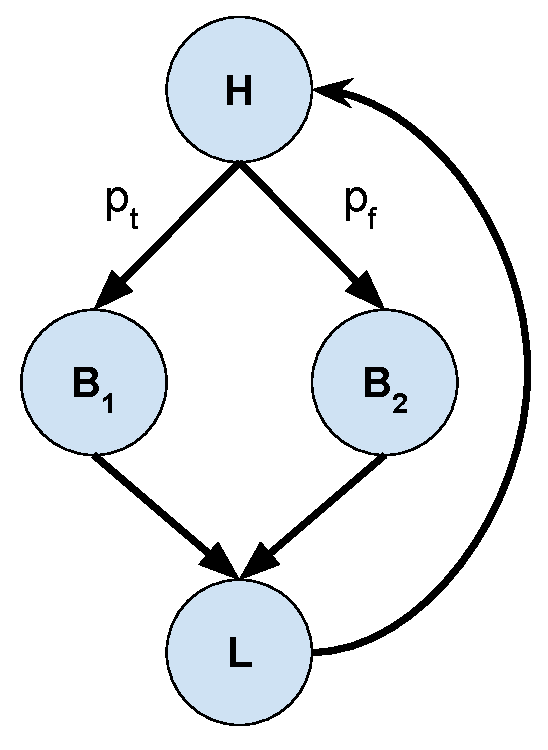
\includegraphics[width=0.9\textwidth, height=.33\textheight]{Figures/02-background/simple-loop-cfg.pdf}
         \caption{Original.}
         \label{fig:simple-loop-cfg}
     \end{subfigure}
     \begin{subfigure}[b]{0.49\textwidth}
         \centering
         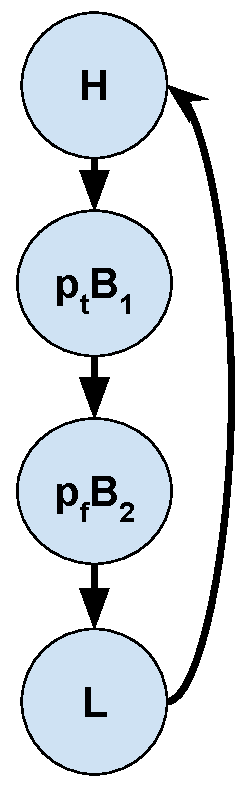
\includegraphics[width=0.4\textwidth, height=.33\textheight]{Figures/02-background/simple-loop-predicated-cfg.pdf}
         \caption{Linearized.}
         \label{fig:simple-loop-predicated-cfg}
     \end{subfigure}\\
     \begin{subfigure}[b]{0.49\textwidth}
         \centering
         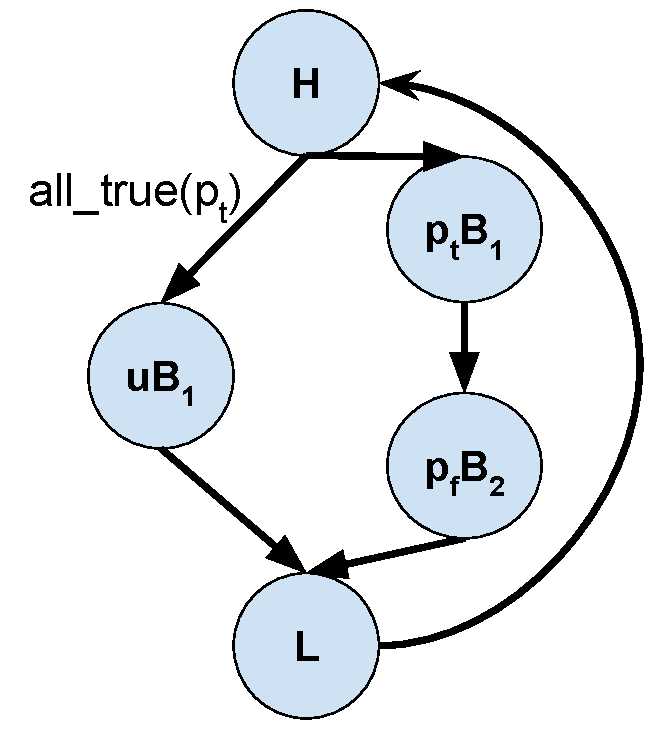
\includegraphics[width=\textwidth, height=.33\textheight]{Figures/02-background/simple-loop-bossc-cfg.pdf}
         \caption{BOSCC.}
         \label{fig:simple-loop-boscc-cfg}
     \end{subfigure}
        \caption{(a) Original CFG of \rlst{simple-loop}; (b) CFG after control-flow linearization (CFL); (c) CFG in (b) after inserting of \code{all\_true} BOSCC.}
        \label{fig:simple-loop-cfgs}
\end{figure}

\section{If-Conversion}
In a loop with \emph{divergent} control flow,  different iterations of the loop may execute instructions from different paths in the loop's \textbf{Control-Flow Graph} (\acrshort{cfg}).
Divergent control flow may be an obstacle to the vectorization of a loop.
Common programming-language constructs, such as \code{if-then-else} and \code{switch-case} statements may introduce divergence.
Modern compilers are able to vectorize some control-flow divergent loops after applying a \textbf{Control-Flow Linearization} (CFL) technique known as \code{If}-Conversion.
If conversion transforms control-flow dependencies into data dependencies \cite{allen_conversion_1983, park1991ifconversion}.
For instance, consider the \code{for}-loop in \rlst{simple-loop} and its CFG in \rfig{simple-loop-cfg}.
The statements on \rline{simple-loop:true-path} and \rline{simple-loop:false-path} are control-flow dependent on the condition in \rline{simple-loop:condition}.
CFL eliminates control flow by first computing a predicate register for each possible path.
Then the instructions on each basic block are guarded with the predicate registers that correspond to the condition that needs to be true for that block to be executed.
For example, instructions in block $B_1$ are predicated with a predicate register $p_t$, where $p_t = (a[i] < b[i])$.
$B_2$ are predicated with a predicate register $p_f$, where $p_f = (a[i] \geq b[i]) = \neg p_t$.
\rfig{simple-loop-predicated-cfg} shows the CFG in \rfig{simple-loop-cfg} after CFL, where predicated blocks are denoted by prefixing the original block name with their corresponding predicate register.


\begin{figure*}[t]
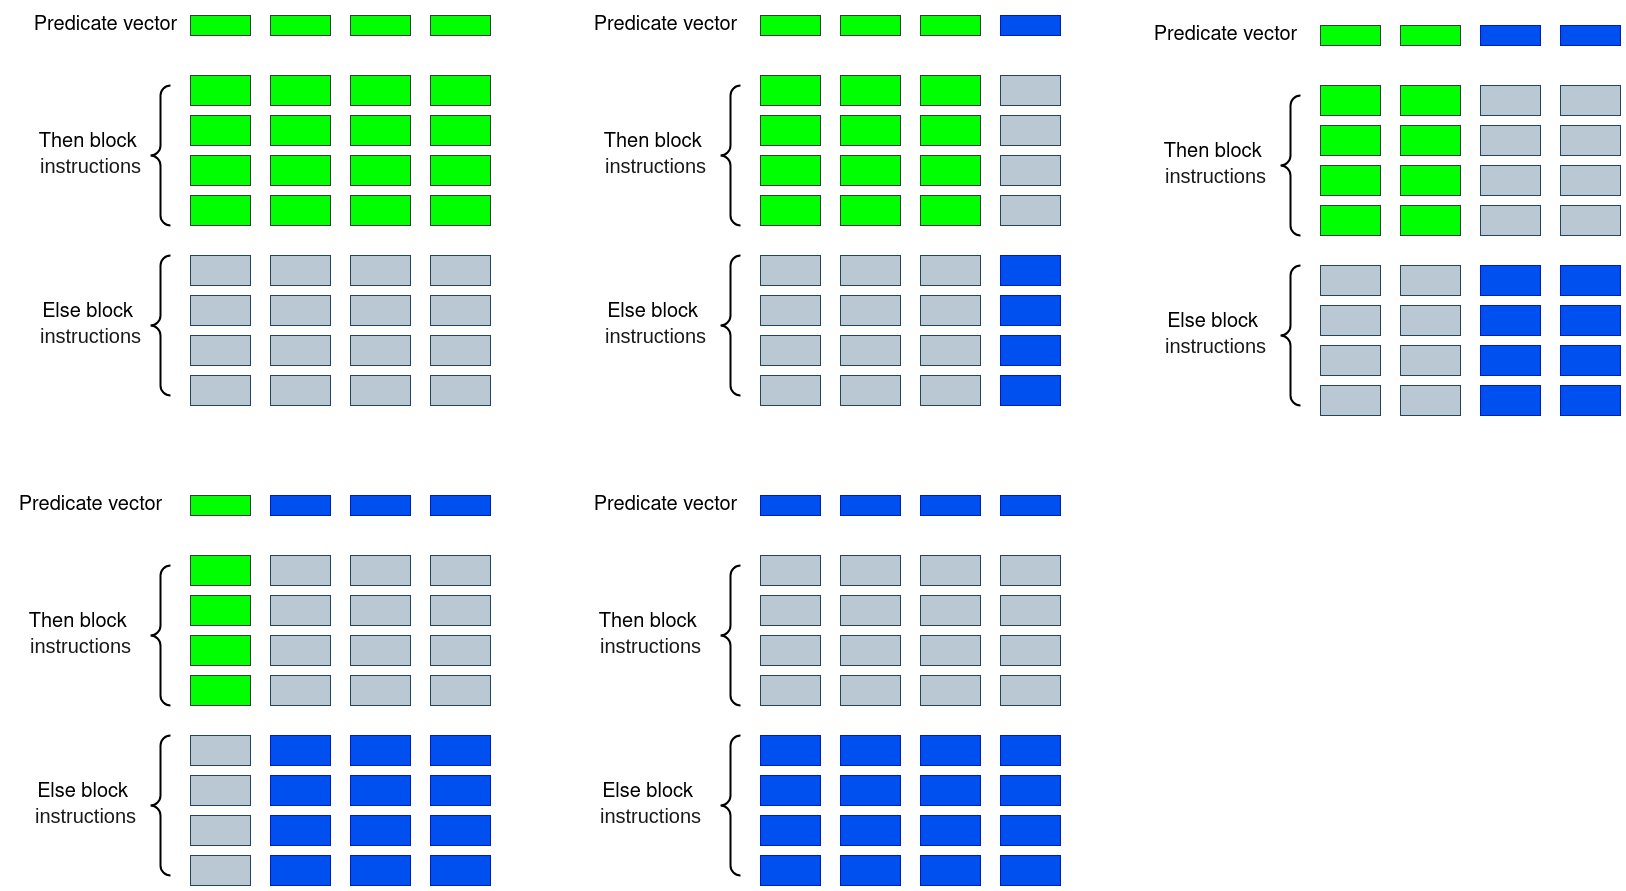
\includegraphics[width=\textwidth]{Figures/02-background/condition_distribution.png}
\centering

\caption{All Possible Condition Distributions for \rlst{simple-loop}. Green elements represent vector lanes executing instructions of the then block, blue ones represent vector lanes executing instructions of the else block, and the gray elements show inactive lanes. }
\label{fig:condition-distribution}
\end{figure*}

Once the body of a loop is linearized via CFL, vectorization proceeds with the conventional recipe followed by most modern compilers, which consists of widening scalar operands into vector operands and replacing scalar operations with their equivalent vector versions.
Scalar predicate registers are replaced with vector predicate registers.
Predicated execution, or simply \emph{predication}, of scalar instructions is supported on modern processors via predicated instructions.
For vector instructions, predication is supported via predicated vector instructions or bit-wise vector instructions, in a process known as \emph{masking}.

Although CFL enables the use of SIMD instructions, it clearly wastes resources and computational cycles because all instructions from each mutually exclusive path will be executed but only one path will have their computations committed.

\rfig{condition-distribution} shows all possible combinations of predicates in each vector loop iteration. As illustrated, regardless of how predicates are distributed among the mask vector, half of the computation power is always lost due to predication (gray elements). This is particularly true when the number of instructions in both the \code{then} and the \code{else} blocks is approximately the same, which is often the case. Furthermore, the problem is even further intensified when we face unbalanced conditions, where we have to execute one of the two paths more than the other one. In such cases, the effect of predication  could become more significant, as we might end up losing more computation power due to a large number of inactive lanes.


\section{Branch-On-Superword-Condition-Codes}

Generating \textbf{Branch-On-Superword-Condition-Codes} (\acrshort{boscc}s) is a common technique to avoid executing instructions from paths where vector lanes would be inactive \cite{ jaewook_shin_superword-level_2005, shin_introducing_2007, shin_evaluating_2009}.
BOSCCs are instructions, or a sequence of instructions, that dynamically checks the uniformity of predicate registers.
In a uniform predicate register the condition evaluates to the same value --- all true or all false --- for all lanes.
In such cases, only the instructions corresponding \emph{uniform path}, true path or false path, need to be executed.
For example, after vectorization, in \rfig{simple-loop-predicated-cfg} if $p_t$ is a uniform true vector, then only instructions in $B_1$ need to be executed and instructions in $B_2$ can be skipped.
\rfig{simple-loop-boscc-cfg} shows the CFG in \rfig{simple-loop-predicated-cfg} after BOSCCs are inserted by the compiler.
As \rfig{simple-loop-boscc-cfg} shows, an \code{all\_true} \emph{guard condition} is generated to check if $p_t$ is a uniform true vector.
In such a case, the control flow is directed to a uniform block $uB_1$, that only contains instructions from block $B_1$.
When $p_t$ is a uniform true vector, the instructions in block $B_2$ can be skipped because $p_f = \neg p_t$, and thus all lanes would be inactive.


\section{Active-Lane-Consolidation}

The insertion of BOSCCs can improve SIMD utilization and reduce the number of wasted cycles by avoiding executing vector instructions with all lanes inactive.
However, the benefits of BOSCCs can only be observed if uniform vectors occur frequently.
If uniformity is rare, then the use of BOSCCs does not increase SIMD utilization \cite{praharenka_vectorizing_2022}.
Moreover, the likelihood of uniformity decreases with increased VL, thus uniform predicate vectors are less likely to be found for architecture with long vectors --- e.g. AVX512 and Fujitsu A64Fx.
\textbf{Active-Lane Consolidation} (ACL) is an algorithm proposed to increase SIMD utilization even in the presence of infrequent uniform vectors and architectures with long vectors \cite{praharenka_vectorizing_2022}.
At the core, ACL is a permutation algorithm that creates uniform vectors by merging active lanes from two, or more, non-uniform vectors into a \emph{merged vector}.
Permutation enables ALC to only execute non-predicated blocks with the constructed uniform vector and effectively avoid executing linearized code.

Praharenka \etal propose ALC as an algorithm and manually apply it to each evaluated benchmark.
This work presents the first compiler-only optimization pass that automatically applies ALC to a loop that contains divergent control flow. 
Furthermore, during the seminal work of Praharenka \etal they had no access to a processor that implements SVE.
Therefore, all their experimental results are based on simulations conducted with the Arm's Instruction Emulator (\acrshort{armIE}) and Praharenka \etal's work only shows improvements in terms of the reduction in the number of executed instructions.
Our performance study on a hardware implementation of SVE revealed that some of the estimates for the latency of instructions used by Praharenka \etal were significantly off.
This work shows that accounting for the actual instruction latencies in a hardware implementation of ALC requires a redesign of aspects of ALC.
To the best of our knowledge, this work is the first to show ALC's performance on real hardware.
Moreover, it identified limitations on the original algorithm that will be discussed in the following chapter.

